\chapter{Fundamentação Teórica}
\label{cap:fundamentacao}
Este capítulo aborda a fundamentação teórica necessária para o profundo entendimento do presente trabalho, bem como do modelo de classificação proposto. Primeiramente é introduzido o conceito de Descoberta de Conhecimento em Banco de Dados. Após, é detalhado o conceito e funcionamento de três algoritmos usados para classificação, são eles: Florestas Aleatórias, Support Vector Machine e Adaboost. 

% --- Descoberta de Conhecimento em Banco de Dados --- %
\section{Descoberta de Conhecimento}
A primeira vez que apareceu o termo \textit{Descoberta de Conhecimento em Banco de Dados} (do inglês \textit{Knowledge Discovery in Database}) foi em 1989, por Piatetsky-Shapiro, com o objetivo de enfatizar que o produto final do processo é o conhecimento.

Para \cite{fayyad:1996} KDD refere-se ao processo geral de descobrir conhecimento útil a partir dos dados, essa extração de conhecimento é um processo não-trivial. 
A Figura ~\ref{fig:kdd} mostra o processo de KDD proposto por Fayyad et al. 
O termo processo implica que o KDD é composto por várias etapas, as quase são iterativas e interativas. 
Iterativa reflete o ciclo entre as etapas e, interativa reflete o caráter interdisciplinar do processo, uma vez que o KDD se aplica em inúmeras áreas e para resolver o problema muitas vezes é necessária a ajuda de um \textit{expert} naquela área.

A seguir, será dada uma visão geral de cada uma das fases.


\begin{figure}
    \centering
    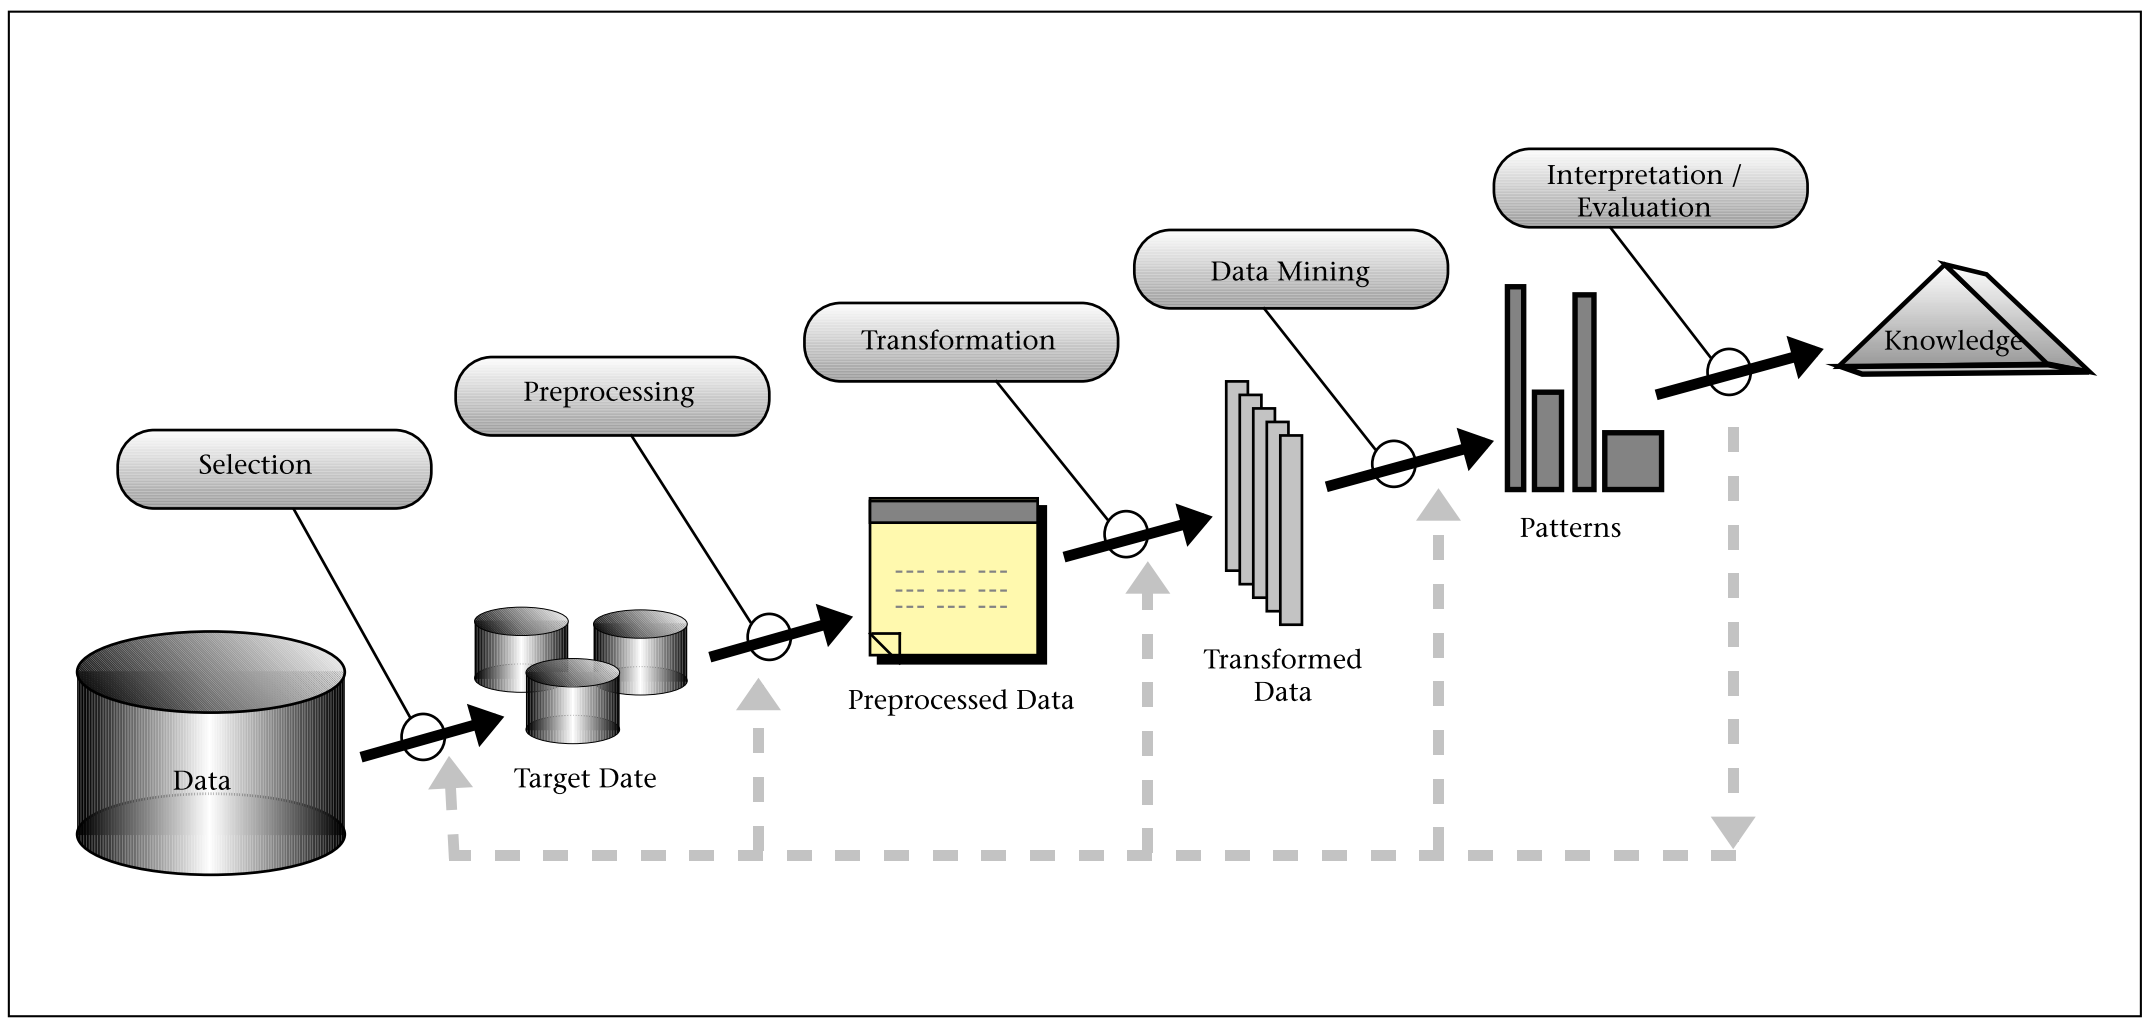
\includegraphics[scale=0.39]{Imagens/kdd.png}
    \caption{Processo de KDD (Fayyad et al)}
    \label{fig:kdd}
\end{figure}

\subsection{Fases do KDD}
% --- SELEÇÃO --- %
\textbf{1) Seleção}: A primeira etapa no processo é chamada de seleção, que é responsável por selecionar um \textit{dataset} a partir de uma base de dados maior. A escolha desse \textit{dataset} dependerá do domínio do problema que está tentando resolver. Em geral, a escolha é feita por um especialista ou por algum algoritmo de extração de características. O conjunto de dados selecionado é chamado de \textit{Target Data}.

% --- PRÉ-PROCESSAMENTO -- %
\textbf{2) Pré-processamento}: Após ter o conjunto de dados a ser utilizado, é comum que esses dados não estejam em boa qualidade, dessa forma, é necessário tratá-los e limpá-los. Operações básicas realizadas nesse nível devem lidar com:

\begin{itemize}[leftmargin=1.2cm]
%    \begin{description}[font=$ \bullet $]
        \item [ Valores faltantes] Valores nulos. Ocorre quando alguém deixa um campo de um formulário em branco, por exemplo.
        \item [ \textit{Outliers}] Quando um valor foge muito do padrão dos dados. Deve ser identificado e eliminado do conjunto de dados.
        \item[ Dados derivados] Ocorre quando um dado pode ser obtido a partir de outro. Por exemplo, a idade de um indivíduo pode ser obtida a partir do seu ano de nascimento, dessa forma, não faz muito sentido ter esses dois atributos no conjunto de dados.
 %   \end{description}
\end{itemize}

% --- TRANSFORMAÇÃO -- %
\textbf{3) Transformação}: Uma vez que os dados estão limpos e tratados, é necessário armazená-los e formatá-los adequadamente para que os algoritmos de aprendizado possam ser utilizados. A título de exemplo, se for usar um algoritmo de agrupamento baseado na distância euclidiana, é necessário converter todos os dados para numérico.

% --- MINERAÇÃO DE DADOS -- %
\textbf{4) Mineração de Dados}:  Embora todas as etapas sejam importantes, a etapa de Mineração de Dados é a que recebe maior atenção. Conforme \cite{fayyad:1996}, mineração de dados é a aplicação de algoritmos específicos para extrair padrões a partir dos dados. Ainda de acordo com Fayyad et al, os algoritmos de mineração de dados podem ser dividimos em cinco categorias: Associação, Classificação, Regressão, Segmentação e Sumarização. A tarefa na qual este projeto se encontra é a de classificação. 

A tarefa de classificação é responsável por identificar a qual classe um determinado registro pertence. Inicialmente, o modelo é ``alimentado'' com conjunto de registros já rotulados, isto é, é fornecida a qual classe os registros pertencem. Com esses dados, o algoritmo treina a aprende padrões que fazem com que um registro pertença a uma classe ou a outra
(esse tipo de aprendizado é conhecido como aprendizado supervisionado).


% -- INTERPRETAÇÃO/VALIDAÇÃO -- %
\textbf{5) Interpretação/Validação}: Uma vez que o modelo já foi treinado, é medido a sua capacidade de generalização. Nesta etapa é fundamental a presença do especialista, visto que, a melhor métrica de avaliação dependerá do negócio. Caso o desempenho não seja satisfatório, é possível retornar para qualquer etapa no processo de KDD, e o ciclo recomeça até chegar a um modelo que satisfaça o negócio.







% --- Ensemble --- %
\section{Ensemble Learning}
\label{sec:ensemble}
Um \textit{ensemble} é composto por um grupo de preditores, que nada mais são do que algoritmos de aprendizado de máquina supervisionados. A técnica de combinar vários preditores é conhecida como \textit{Ensemble Learning} \cite{Geron:2017}. Existem vários métodos baseados nessa estratégia, os mais conhecidos na literatura são: \textit{bagging}, \textit{boosting} e \textit{stacking}.

A figura \ref{fig:ensemble} ilustra um \textit{ensemble} composto por quatro preditores, dos quais três predizeram que uma nova instância é da classe 1 e um preditor disse que a nova instância é da classe 2. Como neste caso, o \textit{ensemble} escolhe a classe de acordo com a votação majoritária de seus preditores, é atribuída a classe 1 à nova instância.

\begin{figure}[ht!]
    \centering
    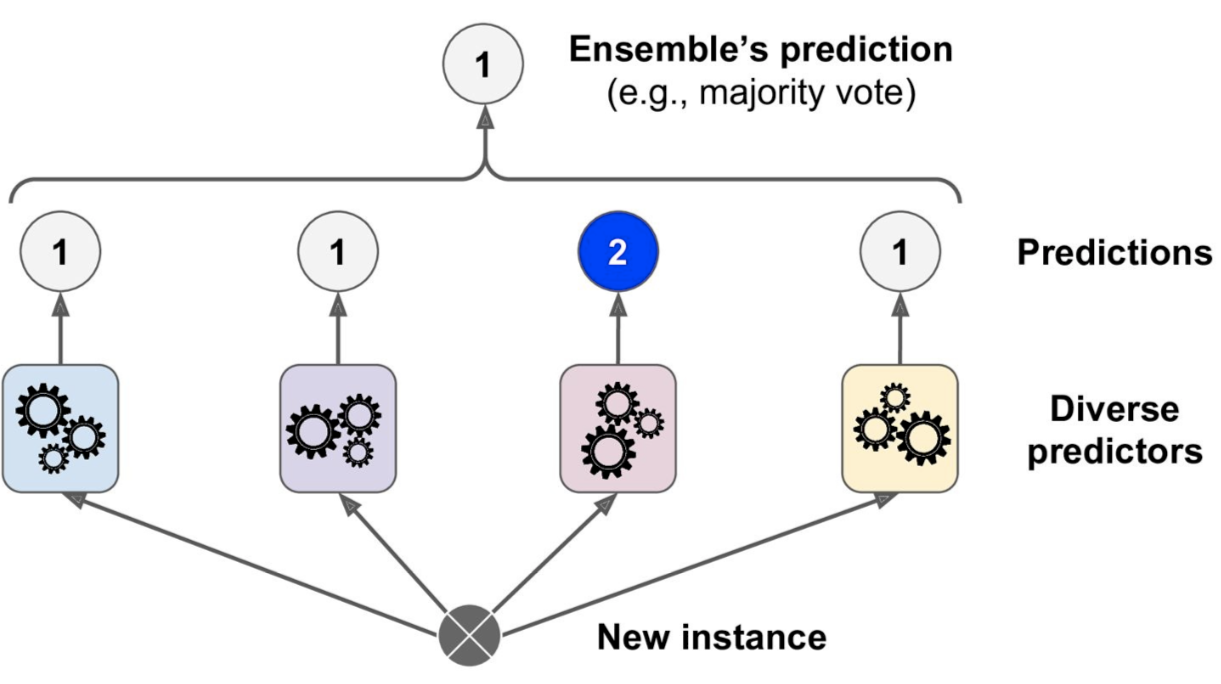
\includegraphics[scale=0.2]{Imagens/ensemble.png}
    \caption{Exemplo de um Ensemble Learning \cite{Geron:2017}}
    \label{fig:ensemble}
\end{figure}

Embora seja mais comum utilizar \textit{Ensemble Learning} para classificação, também é possível utilizar essa técnica para problemas de regressão.

Uma maneira muito simples de agregar os resultados de cada preditor, a fim de chegar em um classificar ainda mais robusto, é escolher a classe com a maior quantidade de votos. Essa estratégia é conhecida como \textit{Hard Voting Classifier} \cite{Geron:2017}.

Contudo, é possível que haja classificadores bons e ruins, caso o número de preditores ruins supere o número de bons, é possível que o método \textit{ensemble} seja prejudicado e tenha um resultado inferior ao melhor preditor. Para contornar esse tipo de problema, uma estratégia possível é atribuir pesos diferentes para os preditores, essa estratégia é conhecida como \textit{Soft Voting Classifier} \cite{Geron:2017}.


\subsection{Bagging e Pasting}
\label{sec:bagging_pasting}
Quando for construir um modelo \textit{ensemble}, uma abordagem possível é utilizar o mesmo algoritmos para treinar os preditores. Contudo, caso os preditores sejam treinados com o mesmo \textit{dataset}, todos os preditores terão o mesmo desempenho, dessa forma, é necessário que os preditores sejam treinados com uma amostra aleatória do conjunto de dados. Caso a amostragem seja feita \textit{com reposição}, esse método é chamado de \textit{bagging} \cite{Breiman_Bagging:1996}. Caso a amostragem seja feita \textit{sem reposição}, o método é chamado de \textit{pasting} \cite{Breiman_Pasting:1999}. 

% --- Florestas Aleatórias --- %
\section{Florestas Aleatórias}

Florestas Aleatórias (do inglês \textit{Random Forest}) é um algoritmo de aprendizado do tipo \textit{ensemble} cujo os meta-classificadores são Árvores de Decisão \cite{Quinlan:1986} treinadas com o método \textit{bagging}.
De acordo com \cite{breiman:2001} a definição formal do algoritmo Floresta Aleatória é dada por:

\begin{definition}\label{def:floresta}
Uma floresta aleatória é um classificador que consiste em uma coleção de classificadores de árvores de decisão ${h(x, \theta _k)}$, onde ${\theta _k}$ são as \textit{features} para o meta-classificador $k$ e, $x$ é o vetor de entrada.
\end{definition}

O algoritmo de Floresta Aleatória introduz um certo nível de aleatoriedade ao treinar os meta-classificadores; em vez de receberem o mesmo conjunto de dados, as árvores de decisão recebem um subconjunto diferente. Por exemplo, na figura \ref{fig:split_floresta} o \textit{dataset} original foi dividido em 2 subconjuntos de dados, os quais serão utilizados para treinar os algoritmos de árvore de decisão. Nota-se que as \textit{features} escolhidas não são as mesmas. Esse processo é importante, pois aumenta a capacidade de generalização do modelo de classificação.

\begin{figure}[h!]
    \centering
    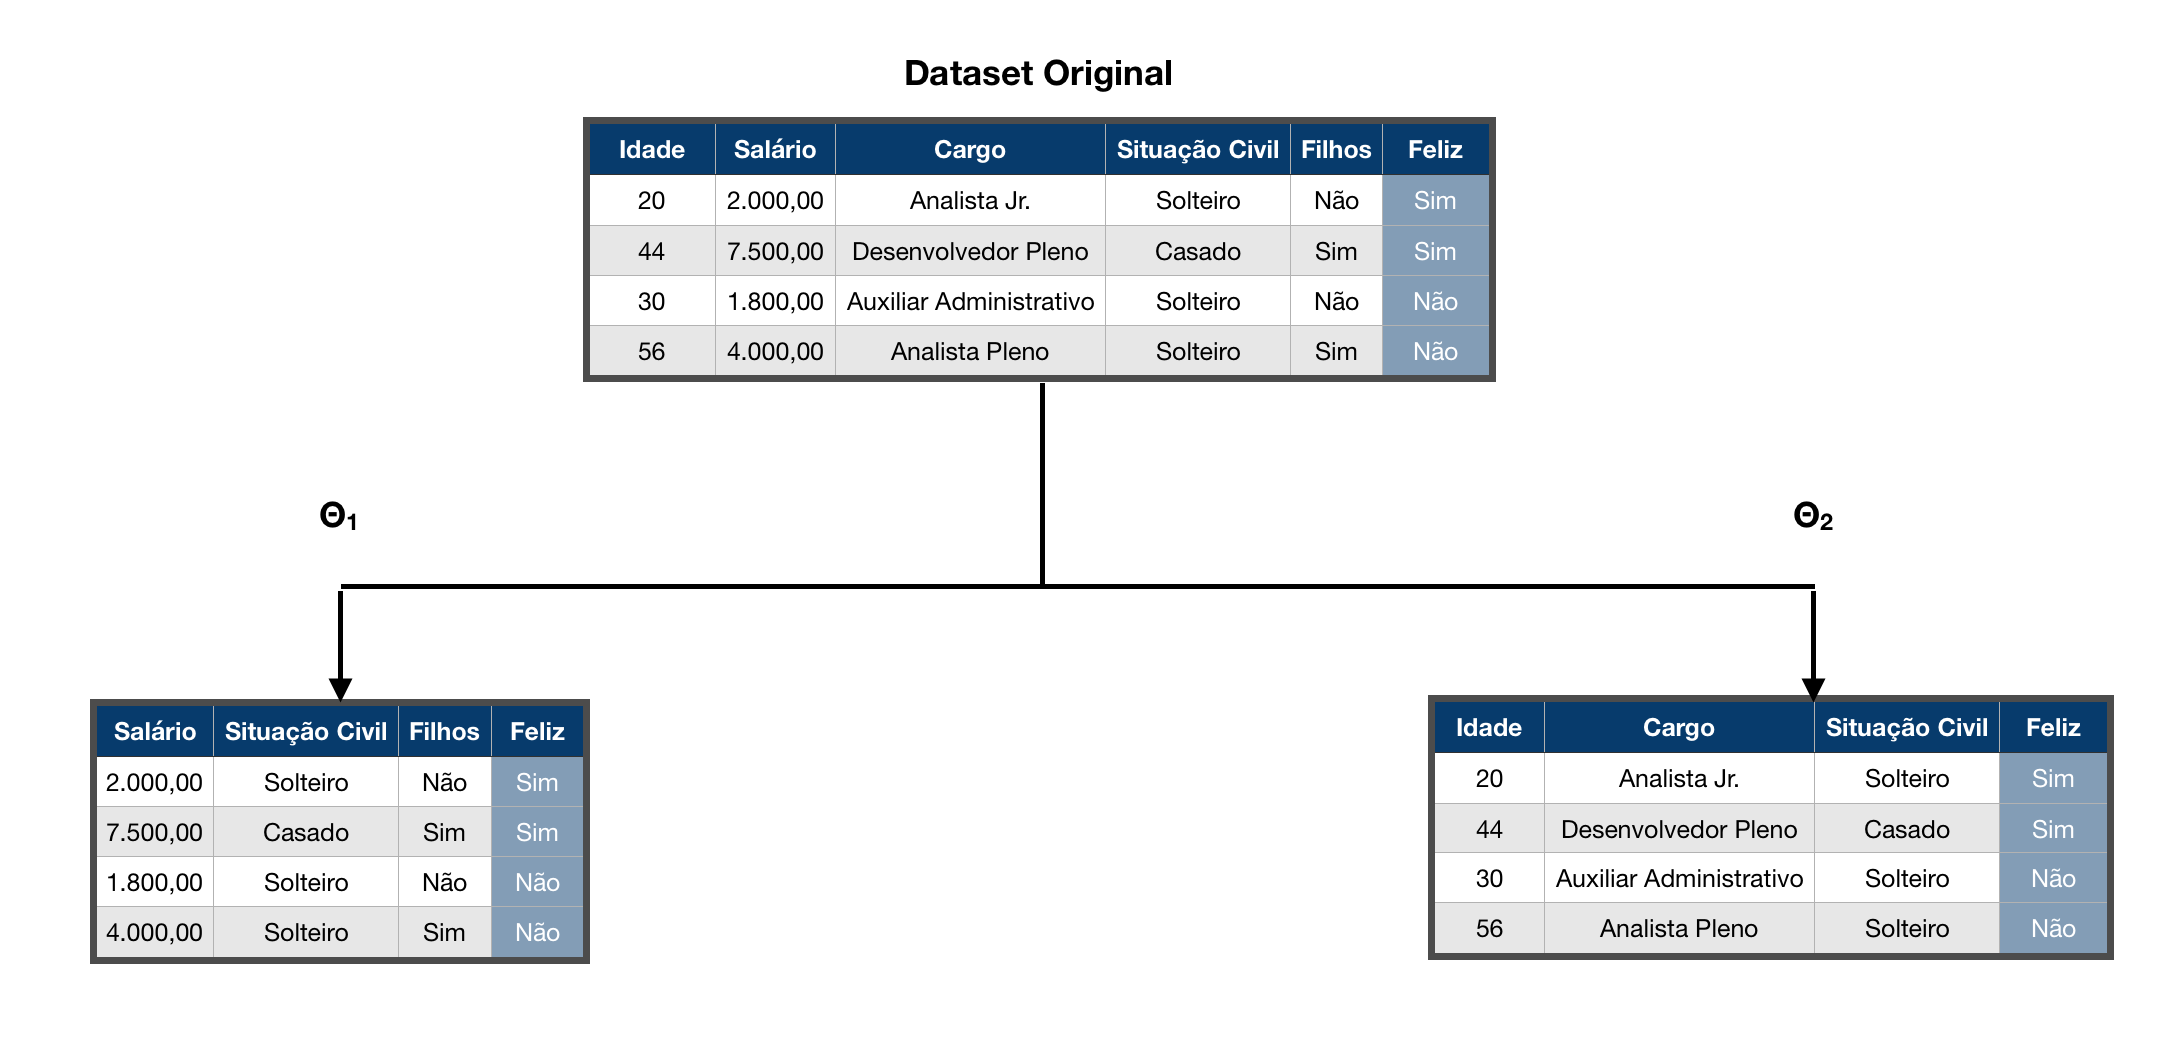
\includegraphics[scale=0.4]{Imagens/split_RandomForest.png}
    \caption{Exemplo de uma divisão randômica do \textit{dataset} original.}
    \label{fig:split_floresta}
\end{figure}

\subsection{A importância das features}
\label{sec:importancia_features}
Uma grande qualidade das florestas aleatórias é o fato de ser possível identificar as melhores \textit{features}, em outras palavras, é possível saber quais são os atributos mais importantes para predizer se um determinado registro irá pertencer a uma classe ou a outra. Se o modelo está sendo treinado para identificar uma doença de acordo com os sintomas, é possível descobrir quais são os sintomas que mais influenciam em um paciente possuir uma determinada doença.


\subsection{Vantagens e Desvantagens}
Um ponto positivo das Florestas Aleatórias é que esse tipo de algoritmo pode ser usado tanto para problemas de classificação quanto para problemas de regressão. 

Como foi dito na sessão \ref{sec:importancia_features}, é possível visualizar a importância de cada \textit{feature}, a fim de compreender melhor o comportamento dos dados e interpretar o modelo aprendido.

Um grande problema que aflige alguns algoritmos de aprendizado supervisionado é o \textit{overfitting}, isto ocorre quando um modelo aprende muito bem o conjunto de treino e sua capacidade de generalização fica comprometida por conta disso. Na maioria das vezes, esse problema não irá acontecer com o modelo de Floresta Aleatória.

A grande desvantagem do modelo de Floresta Aleatória fica por conta da sua performance quando há uma grande quantidade de árvores. Por um lado, quanto mais meta-classificadores melhor tende a ser a acurácia do modelo. Por outro lado, se há muitos meta-classificadores, a performance do algoritmo fica bastante comprometida.

% --- Adaboost --- %
\section{AdaBoost}

O modelo \textit{boosting} refere-se a um método \textit{ensemble} (sessão \ref{sec:ensemble}) para resolver problemas de classificação e regressão. A ideia geral do \textit{boosting} é  combinar vários meta-algoritmos fracos em um modelo robusto. Esses meta-algoritmos são treinados em sequência, onde cada um tenta corrigir seu antecessor \cite{Kearns:1988}.

O algoritmo do tipo \textit{boosting} mais conhecido na literatura é o \textit{Adaptive Boosting} ou simplesmente \textit{AdaBoost}, que foi proposto por \cite{Freund:1997}. O algoritmo pode ser usado para melhorar o desempenho de qualquer algoritmo de \textit{machine learning}. Contudo, AdaBoost funciona melhor com preditores fracos \footnote{Preditores fracos são aqueles que alcançam uma acurácia pouco acima de um preditor aleatório.}.

O preditor mais comum para ser usado com o AdaBoost são as árvores de decisão com um nível. Pelo fato dessas árvores possuírem apenas um nível, são conhecidas na literatura como \textit{Decision Stump} (algo como Toco de Decisão, em vez de Árvore de Decisão).

\subsection{Funcionamento}
O trabalho de \cite{Freund:1999} foi utilizado como referência para a explicação do funcionamento do algoritmo que será dada a seguir.

Inicialmente, é fornecido como entrada para o algoritmo, o conjunto de treino $(x_1, y_1), (x_2, y_2) ..., (x_m, y_m)$, onde cada $x_i$ pertence ao conjunto de instâncias $X$, e cada $y_i$ pertence ao conjunto de rótulos $Y$. Para problemas envolvendo a classificação binária (ou dicotômica), considera-se $Y = \{-1, +1\}$. 

Adaboost utiliza $T$ preditores, os autores chamam os preditores de \textit{hipóteses}, denotando as hipóteses como sendo $h_1(x), h_2(x),..., h_T(x)$, onde $x$ representa uma instância a ser classificada pela hipótese (preditor) $h_t(x)$.

Uma das principais ideias do algoritmo é manter uma distribuição ou conjunto de
pesos sobre o conjunto de treinamento. Isto é, cada instância no conjunto de treinamento existe um peso associado e, a medida que o algoritmo evolui, quanto mais difícil for para classificar uma instância de treinamento, maior será o peso atribuído a ela. De modo que, para os preditores subsequentes, a chance de classificar corretamente esse dado é maior. O peso dessa distribuição para um dado de treinamento $i$ na rodada $t$ é denotado por $D_t(i)$.

Inicialmente, todas as instâncias no conjunto de treinamento possuem exatamente o mesmo peso $w_i = \dfrac{1}{N}$, onde $N$ é o tamanho do conjunto de treinamento. Mas, a cada rodada, o peso das amostras classificadas erroneamente são aumentados, dessa forma, os preditores são forçados a focar nas amostras mais difíceis de serem classificadas.




% --- Support Vector Machine --- %
\section{SVM}

Máquinas de Vetores de Suporte, do inglês \textit{Support Vector Machines}, é um tipo de algoritmo de Aprendizado de Máquina supervisionado, utilizado para problemas de classificação envolvendo duas ou mais classes. O algoritmo foi proposto por \cite{Cortes:1995}. 

A ideia do SVM é mapear vetores de entrada em alguma dimensão maior, através de algum mapeamento não-linear, escolhido a piori. Neste novo espaço um hiperplano é construído para separar os dados \cite{Cortes:1995}.

\begin{figure}[ht!]
    \centering
    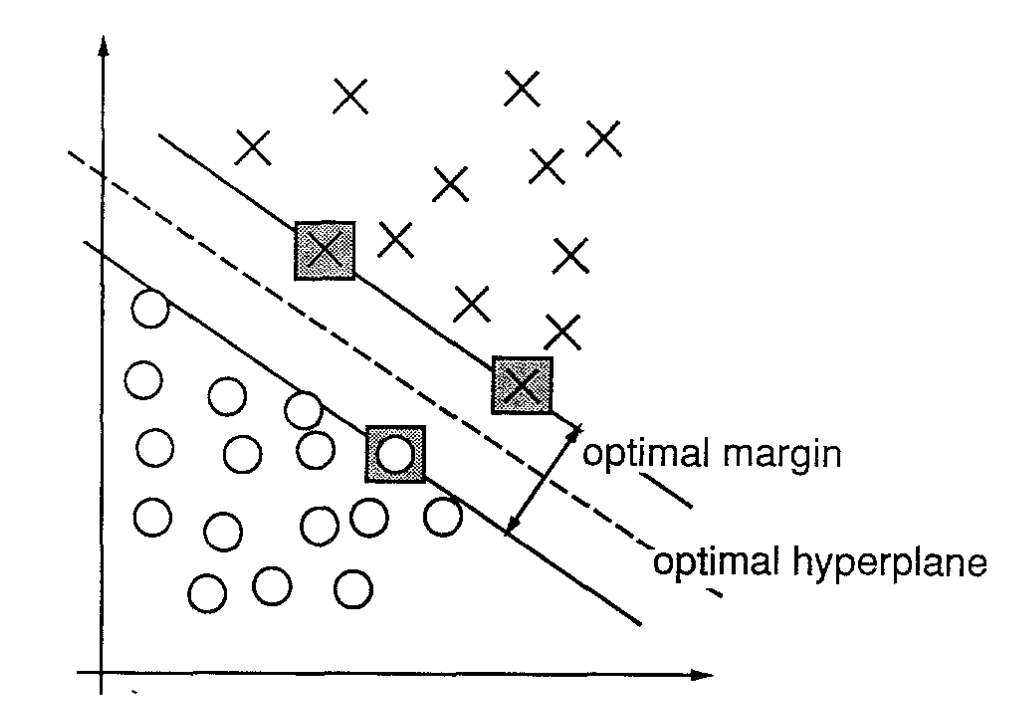
\includegraphics[scale=0.70]{Imagens/svm-exemplo.png}
    \caption{Um exemplo de um conjunto de dados linearmente separável em duas dimensões. \cite{Cortes:1995}}
    \label{fig:svm-exemplo}
\end{figure}

A figura \ref{fig:svm-exemplo} mostra um conjunto de dados que pode ser separado de maneira linear. O objetivo do SVM é encontrar o melhor hiperplano, de maneira que a margem\footnote{Margem é o dobro da distância entre o hiperplano e o ponto mais perto} seja a maior possível. 

\subsection{Vantagens e Desvantagens}
Um \textit{Support Vector Machine} é um modelo de classificação poderoso e versátil, capaz de realizar classificação linear e não linear, regressão e até detecção de \textit{outliers}. SVMs são parcularmente bem adequadas para problemas de classificação complexo, porém com \textit{datasets} não muito grandes \cite{Geron:2017}.

Um lado negativo do SVM é sua sensibilidade à escala dos dados de entrada. A figura \ref{fig:svm-escala} ilustra bem esse problema: no desenho da esquerda, aonde $x_0$ e $x_1$ estão em escalas diferentes, a margem é bem pequena. Quando os dados são normalizados, como mostra no desenho da direita, a margem fica bem maior, possibilitando melhor generalização na hora de classificar novas instâncias.

\begin{figure}[ht!]
    \centering
    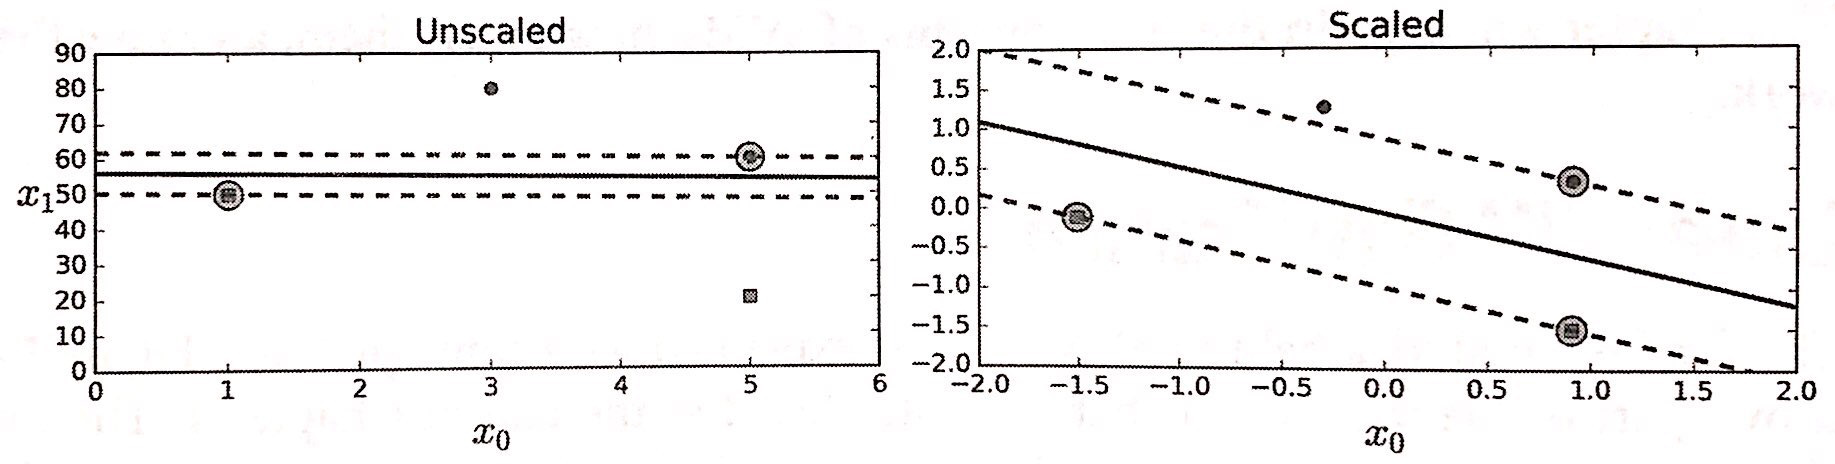
\includegraphics[scale=0.25]{Imagens/smv_escala.png}
    \caption{Sensibilidade com a escala dos dados \cite{Geron:2017}}
    \label{fig:svm-escala}
\end{figure}

